\section{Introduction}\label{sec:intro}

Persistent homology summarizes the shape of data by the cycles of a simplicial complex and the scales at which they appear and disappear~\cite{ELZ02,ZC05,EH10}.
In a growing number of applications the complex is not fixed but changes over time.
Examples include collective motion and other time-varying point clouds~\cite{TZH15,KM21}, sliding-window embeddings of signals~\cite{PH15}, streaming data, where complexes evolve by insertions and edge contractions~\cite{KS19}, and gradient-based optimization and learning, where the complex or its filtration changes at every step~\cite{HKND19,CCGIKU21}.
Recomputing persistent homology from scratch takes $O(n^{\omega})$ time for a complex with $n$ simplices~\cite{MMS11}, where $\omega<2.372$ is the exponent of matrix multiplication~\cite{ADVXXZ25}.
So a natural goal is a data structure that absorbs a local change, such as the insertion or deletion of one simplex, in time much smaller than~$n$.

The $p$-th Betti number $\beta_p$ of a complex counts its independent $p$-dimensional holes: $\beta_0$ counts connected components, $\beta_1$ independent loops, and $\beta_2$ enclosed voids.
For $\beta_0$ the goal of fast updates has been reached.
The number~$\beta_0$ of connected components is maintained by dynamic connectivity in polylogarithmic time per update~\cite{HDT01,WN13,KKM13}, and Dey, Hou, and Parsa~\cite{DHP23} update the persistence of graph filtrations in sublinear time by maintaining minimum spanning forests in dynamic trees.
For time series, the banana trees of Cultrera di Montesano et al.~\cite{CEHO24} support insertions, deletions, cuts, and concatenations in time logarithmic in the length of the series plus the number of changes to the augmented persistence diagram.
For general complexes of dimension two or more, the update procedures we know of take time polynomial in~$n$ per insertion or deletion of a simplex in the worst case.
Vines and vineyards~\cite{CEMS06} process a transposition of two consecutive simplices in $O(n)$ time, but moving one simplex may take up to $n-1$ transpositions; updates of zigzag persistence, which allows deletions as well as insertions~\cite{DH21u}, warm-started reductions~\cite{LN21}, and recomputation are also polynomial in the worst case.
Is this a shortcoming of the algorithms, or is maintaining homology inherently hard?
We show that the answer is tied to a classical open problem: maintaining Betti numbers is equivalent, up to constant factors, to maintaining the rank of a sparse matrix (an arbitrary one over~$\Ftwo$, and one with entries in $\{0,\pm1\}$ over other fields).
As a consequence, under the Online Matrix--Vector multiplication (\OMv) conjecture~\cite{HKNS15}, for no $\eps>0$ can a data structure with polynomial preprocessing time maintain a Betti number $\beta_p$ with $p\ge1$ under insertions and deletions in amortized time $O(n^{1/2-\eps})$ per update while answering queries in time $O(n^{1-\eps})$.
In the \OMv\ problem, an algorithm receives a Boolean $\ell\times\ell$ matrix~$M$, then Boolean vectors $v_1,\dots,v_\ell$ arrive one at a time, and it must output the Boolean product $Mv_t$ before $v_{t+1}$ is revealed; the conjecture states that no algorithm does this in total time $O(\ell^{3-\eps})$ for any $\eps>0$, that is, polynomially faster than computing every product naively.
It is the standard source of tight conditional lower bounds for dynamic problems~\cite{HKNS15}.
Our bounds concern insertions, deletions, and value changes; they say nothing about the cost of a single transposition (Section~\ref{sec:related}).

\paragraph{The problem.}
We study the following basic problem, defined formally in Section~\ref{sec:prelim}.
A fixed simplicial complex~$\cU$ with $n$ simplices, the \emph{universe}, is given in advance.
A data structure maintains a subcomplex $K\subseteq\cU$ under the insertion and deletion of single simplices and, on request, reports the $p$-th Betti number $\beta_p(K)=\dim H_p(K;\F)$ over a fixed field~$\F$.
We call this problem \emph{dynamic Betti numbers}.
It is the simplest dynamic question one can ask about homology, because the answer is a single integer.
In persistence, a monotone function on the simplices defines a \emph{filtration} by its sublevel sets, the \emph{barcode} records the interval of values during which each homology class lives, and a \emph{persistent Betti number} counts the bars that contain given values.
In particular, $\beta_p(K)$ is the persistent Betti number, at value~$0$, of the function that is $0$ on~$K$ and $1$ elsewhere, so a data structure that maintains a barcode under changes of function values and can count the bars containing a given value also solves dynamic Betti numbers (Lemma~\ref{lem:sublevel}); our lower bounds therefore apply to it.

\subsection{Our results}

Our main finding is that dynamic Betti numbers are a disguised form of a classical problem in dynamic linear algebra: \emph{dynamic matrix rank}, in which one maintains the rank of a matrix under changes of single entries~\cite{FF09,San07,vdBNS19}.

\paragraph{Rank-completeness.}
We call a dynamic problem \emph{rank-complete} if it and dynamic matrix rank reduce to each other with constant overhead per operation and a linear change in instance size (Section~\ref{sec:prelim}); over $\Ftwo$ this refers to the rank of arbitrary matrices, and over other fields to matrices with entries in $\{0,\pm1\}$.
We show that dynamic $\beta_p$ is rank-complete for every fixed $p\ge1$; dynamic $\beta_0$, which is dynamic connectivity, is not, unless the \OMv\ conjecture fails.
One direction is folklore: $\beta_p(K)$ is determined by the ranks of two boundary matrices, and inserting or deleting a simplex changes one column of one of them (Lemma~\ref{lem:betti-to-rank}).
Our first contribution is the converse, with constant overhead.
We use a slightly richer version of dynamic rank (Problem~\ref{prob:rank}).
Besides changing an entry, an update may \emph{switch} a whole row or column off, which removes it from the matrix whose rank is queried, or switch it back on.
A set of \emph{admissible positions}, fixed in advance, contains every position that may ever hold a nonzero entry, so that the size of an instance can reflect sparsity.

\begin{theorem}[informal version of Theorem~\ref{thm:equiv} and Corollary~\ref{cor:equiv}]\label{thm:intro-equiv}
Let $\F$ be a field.
\begin{enumerate}[label=(\roman*)]
\item Maintaining the rank of a $0/1$ matrix over~$\F$ with $r$ rows, $k$ columns, and $m$ admissible positions, under entry flips and switches, reduces to maintaining $\beta_1$ of a $2$-complex with $O(r+k+m)$ simplices: an entry flip costs seven simplex insertions or deletions, a switch costs one, and a rank query costs one Betti query. For matrices with entries in $\{0,\pm1\}$, an entry update costs at most eight simplex updates.
\item Conversely, for every fixed $p\ge0$, maintaining $\beta_p$ of a subcomplex of a universe with $n$ simplices reduces to maintaining the rank of a matrix with entries in $\{0,\pm1\}$ and $O(n)$ admissible positions, with one switch per simplex update.
\end{enumerate}
\end{theorem}

Theorem~\ref{thm:intro-equiv} shows that over $\Ftwo$, dynamic $\beta_1$ of $2$-complexes and dynamic matrix rank are equivalent up to constant factors in time and size; over every field, the same holds for matrices with entries in $\{0,\pm1\}$, which include all boundary matrices (Section~\ref{sec:equiv-thm}).
Size here is the instance size $N=r+k+m$ of Problem~\ref{prob:rank}, not the dimension of the matrix: a dense $s\times s$ matrix becomes a complex with $\Theta(s^2)$ simplices.
This measure matters when comparing bounds: the hard instances of our lower bound (Theorem~\ref{thm:intro-omv} below) encode dense $\sqrt n\times\sqrt n$ matrices, on which the dynamic-rank algorithm of van den Brand, Nanongkai, and Saranurak~\cite{vdBNS19} takes $O(n^{0.7035})$ time per update, whereas on the boundary matrices of an arbitrary complex it takes $O(n^{1.407})$ time (Corollary~\ref{cor:upper}); the remaining gap is inherited from dense dynamic rank.

The reduction rests on a local, switchable gadget (Figure~\ref{fig:gadget} and Section~\ref{sec:overview}).
It follows the pattern of the static reduction of Edelsbrunner and Parsa~\cite{EP14}, with rows and columns exchanged: rows become hollow triangles, columns become punctured spheres, and the $2$-cycles encode the linear dependencies among the columns, so $\beta_2$ equals the nullity of the matrix and $\beta_1$ follows from the Euler--Poincar\'e formula.
Edelsbrunner and Parsa only need some triangulation with $O(h)$ simplices of each sphere with $h$ holes, and such a triangulation may change in $\Theta(h)$ simplices when a hole is added or removed; on dense matrices, $h=\Theta(\sqrt n)$.
We add two features.
\emph{Switches}, one triangle each, turn rows and columns off and on; they alone already yield the basic \OMv\ lower bound (Theorem~\ref{thm:intro-omv} below).
And we assemble every punctured sphere from constant-size pieces, one per admissible position, so that every entry update costs a constant number of simplex updates; this locality yields the equivalence.
Switches alone suffice for the basic lower bound and most of its variants, and they could equally be added to the static complex of~\cite{EP14}; constant-cost entry updates are needed for the equivalence itself and for the results that flip entries, namely the worst-case bounds (Theorem~\ref{thm:worstcase} and Corollary~\ref{cor:hinted}) and the hardness of deciding whether $H_1$ vanishes (Theorem~\ref{thm:acyclic}).

% Figure: the gadget K(A), schematic overview (details in fig-socket.tex).
% Requires tikz with the patterns library. Okabe--Ito colors: rows vermillion, columns blue.
\begin{figure}[t]
\centering
\definecolor{gRow}{HTML}{D55E00}%
\definecolor{gCol}{HTML}{0072B2}%
\colorlet{gLine}{gCol!80!black}%
\tikzset{
  gsurf/.style={fill=gCol!10,draw=gLine,line width=0.6pt},
  gtube/.style={double=gCol!24,double distance=4.4pt,line width=0.55pt,draw=gLine},
  growcyc/.style={draw=gRow,line width=1.15pt,line join=round},
  gseal/.style={fill=black!72,draw=black,line width=0.4pt},
  ghole/.style={fill=white,draw=gLine,line width=0.5pt},
  gteth/.style={fill=black!28,draw=black!80,line width=0.75pt,line join=round},
  glab/.style={font=\small},
  gsmall/.style={font=\footnotesize},
  gpanel/.style={font=\small}}
\providecommand\Description[2][]{}%
\Description{Schematic of the gadget for a two-by-three matrix: two orange hollow triangles (row cycles) at the top, three blue spheres (column surfaces) at the bottom, blue tubes joining a hole of each sphere to the row cycles of the rows in which the column has a one, dark seals on the other holes, and a gray tether triangle below each sphere.}
\begin{tikzpicture}[x=1cm,y=1cm]
  %%% (a) the complex K(A) for a 2 x 3 matrix
  \node[glab] at (0.95,2.55) {$A=\begin{pmatrix}\textcolor{gLine}{\mathbf 1}&\textcolor{gLine}{\mathbf 1}&\textcolor{black!45}{0}\\ \textcolor{black!45}{0}&\textcolor{gLine}{\mathbf 1}&\textcolor{gLine}{\mathbf 1}\end{pmatrix}$};
  % tubes of the 1-entries (drawn first; surfaces and row cycles cover their ends)
  \draw[gtube] (3.18,0.98) .. controls (3.25,2.05) and (4.3,2.3) .. (4.43,2.98);
  \draw[gtube] (5.48,0.98) .. controls (5.41,2.05) and (4.8,2.3) .. (4.67,2.98);
  \draw[gtube] (5.92,0.98) .. controls (5.99,2.05) and (6.6,2.3) .. (6.73,2.98);
  \draw[gtube] (8.22,0.98) .. controls (8.15,2.05) and (7.1,2.3) .. (6.97,2.98);
  % tubes to the tethers
  \foreach \x in {3.4,5.7,8.0} \draw[gtube] (\x,0.1) -- (\x,-0.62);
  % column surfaces
  \foreach \x/\j in {3.4/1,5.7/2,8.0/3} {
    \draw[gsurf] (\x,0.52) ellipse (0.9 and 0.54);
    \fill[white,opacity=0.55] (\x-0.4,0.74) ellipse (0.2 and 0.085);
    \node[glab] at (\x,0.38) {$\Sigma_{\j}$};
  }
  % holes: tubed (white rim) and sealed (dark)
  \foreach \x in {3.18,5.48,5.92,8.22} \draw[ghole] (\x,1.0) ellipse (0.13 and 0.05);
  \foreach \x in {3.62,7.78} \draw[gseal] (\x,0.99) ellipse (0.15 and 0.065);
  % row cycles (hollow triangles: both rows active)
  \foreach \x/\i in {4.55/1,6.85/2} {
    \draw[growcyc] (\x-0.36,2.98) -- (\x+0.36,2.98) -- (\x,3.52) -- cycle;
    \node[glab,text=gRow] at (\x,3.8) {$C_{\i}$};
  }
  % tethers with their fillings E_j (filled: column active)
  \foreach \x/\j in {3.4/1,5.7/2,8.0/3} {
    \draw[gteth] (\x-0.3,-0.62) -- (\x+0.3,-0.62) -- (\x,-1.08) -- cycle;
    \node[gsmall] at (\x+0.58,-0.86) {$\Lambda_{\j}$};
  }
  % legend of (a)
  \begin{scope}[shift={(9.35,1.05)}]
    \draw[gtube] (0,1.0) -- (0.5,1.0); \node[gsmall,anchor=west] at (0.6,1.0) {tube: $A_{ij}=1$};
    \draw[gseal] (0.25,0.5) ellipse (0.15 and 0.065); \node[gsmall,anchor=west] at (0.6,0.5) {seal: $A_{ij}=0$};
    \draw[gteth] (0.1,0.13) -- (0.4,0.13) -- (0.25,-0.13) -- cycle; \node[gsmall,anchor=west] at (0.6,0.0) {filled tether};
  \end{scope}
\end{tikzpicture}
\caption{The gadget $\KA$ for a $2\times3$ matrix~$A$, drawn schematically.
Row~$i$ becomes a hollow triangle, the \emph{row cycle}~$C_i$.
Column~$j$ becomes a surface~$\Sigma_j$, drawn as a sphere with one hole per admissible position (here every position is admissible) and one more hole, which is tubed to its \emph{tether}~$\Lambda_j$.
The hole of row~$i$ is tubed to~$C_i$ if $A_{ij}=1$ and sealed if $A_{ij}=0$; the tubes and seals belong to~$\Sigma_j$.
Filling a row cycle switches its row off, and filling a tether, as drawn, switches its column on.
Here $\rk A=2$, and over~$\Ftwo$ the only nonzero $2$-cycle consists of the three surfaces and the three filled tethers; it encodes the fact that the three columns of~$A$ sum to zero, so $\beta_2(\KA)=3-\rk A=1$.
Figure~\ref{fig:socket} shows how each surface is assembled from constant-size pieces.}
\label{fig:gadget}
\end{figure}


\paragraph{Conditional lower bounds.}
Dynamic rank with switches is hard under the \OMv\ conjecture by an elementary argument: for Boolean vectors $u,v$, the Boolean product $u^{\top}Mv$ equals~$1$ exactly when the submatrix $M[\supp u,\supp v]$ formed by the rows in the support $\supp u=\{i:u_i=1\}$ and the columns in the support $\supp v$ is nonzero, that is, has rank at least one (Lemma~\ref{lem:rank-omv}).
Because our gadget implements every switch with a single simplex update, this hardness transfers to Betti numbers, deterministically and over every field.

\begin{theorem}[informal version of Theorem~\ref{thm:omv} and Corollaries~\ref{cor:allp} and~\ref{cor:persistence}]\label{thm:intro-omv}
Assume the \OMv\ conjecture, and let $\F$ be a field, $p\ge1$, and $\eps>0$.
No data structure with polynomial preprocessing time maintains $\beta_p(K;\F)$ of a subcomplex $K$ of a given universe of dimension $\max\{p,2\}$ with $n$ simplices under simplex insertions and deletions with amortized update time $O(n^{1/2-\eps})$ and query time $O(n^{1-\eps})$.
The same holds for persistent Betti numbers of the sublevel-set filtration of a monotone function on a fixed complex, under updates that change one function value at a time, already for $\{0,1\}$-valued functions.
\end{theorem}

The hard universes form one explicit family; by Theorem~\ref{thm:intro-dichotomy}(i) below, the bound does not hold for universes in~$\R^3$.

\paragraph{Robustness.}
The lower bound of Theorem~\ref{thm:intro-omv} survives each of the following restrictions, and it extends to related problems (Section~\ref{sec:lower}).
\begin{itemize}
\item \emph{Bounded degree.} Every vertex of the universe lies in a constant number of simplices (Theorem~\ref{thm:bdeg} and Corollary~\ref{cor:bdeg-allp}).
\item \emph{Geometry.} The universe is a fixed $2$-complex that is linearly embedded in~$\R^4$, that is, its triangles are straight triangles that meet only in common edges and vertices; this holds for $\beta_1$ and~$\beta_2$ (Theorem~\ref{thm:r4}).
\item \emph{Point clouds and metric spaces.} The complex is a clique complex (the complex of all cliques of a graph) under vertex or edge updates, the Vietoris--Rips complex (all sets of points with pairwise distances at most~$1$) of a finite metric space whose distances change one at a time, or the Vietoris--Rips complex of a point set in $\R^{O(\log n)}$ under point insertions and deletions; the query asks for $\beta_1$ (Theorem~\ref{thm:flag}) or, by the same argument, for $\beta_p$ with any fixed $p\ge2$, and $n$ is the number of vertices or points.
\item \emph{Almost no homology.} The query only asks whether $H_1(K)=0$, on connected complexes with $\beta_1=\beta_2\le1$ (Theorem~\ref{thm:acyclic}). So neither algorithms whose running time depends on the size of the answer nor algorithms that approximate $\beta_1$ within any factor can beat the bound on all inputs.
\item \emph{Zigzag persistence.} A sequence of simplex insertions and deletions is a \emph{zigzag filtration}, and its degree-one barcode records the interval of steps during which each independent loop lives. An online algorithm that reports it for filtrations of length~$L$ needs total time $L^{3/2-o(1)}$ (Corollary~\ref{cor:zigzag}).
\item \emph{Partially dynamic.} The data structure supports only insertions, or only deletions; here the bound is for worst-case update time (Theorem~\ref{thm:partial}).
\end{itemize}

\paragraph{Relation to dynamic rank.}
For dynamic rank itself, \OMv-hardness over large fields was observed by van den Brand, Nanongkai, and Saranurak~\cite{vdBNS19}.
For row and column updates, it follows from~\cite[Theorem~E.5]{vdBNS19full}: \OMv-hardness of $st$-reachability under node updates~\cite{HKNS15} transfers to bipartite perfect matching under node updates~\cite{AV14}, whose size is, with high probability, the rank of the biadjacency matrix with random entries~\cite[Theorem~C.24]{vdBNS19full}.
Lemma~\ref{lem:rank-omv} instead gives a direct and deterministic reduction from \OuMv\ (the variant of \OMv\ whose requests are pairs $(u,v)$ of Boolean vectors, answered by the Boolean value $u^{\top}Mv=\bigvee_{i,j}u_iM_{ij}v_j$, not its parity) over every field, using switches or, equivalently, the padding identity~\eqref{eq:padding}.
On the side of rank, the bounded-degree version of our gadget shows that over every field, dynamic rank under entry updates is \OMv-hard already for matrices with entries in $\{0,\pm1\}$ and at most three admissible positions in every row and column (Corollary~\ref{cor:sparse-rank}); this also follows without topology from Lemma~\ref{lem:rank-omv} and an elementary dynamic sparsification by partial sums, and static sparsifications of this kind are known~\cite{EP14,Yus08}.

\paragraph{Worst-case bounds and algorithms.}
Worst-case lower bounds for dynamic rank of dense $\ell\times\ell$ $0/1$ matrices under entry flips transfer to Betti numbers through the equivalence, with the exponent halved because the universe has $n=\Theta(\ell^2)$ simplices (Theorem~\ref{thm:worstcase}).
Combining this transfer with the hinted variants of \OMv\ proposed by van den Brand et al.~\cite{vdBNS19}, in which information about the future query vectors is revealed in advance, we show that over every field, every data structure with polynomial preprocessing time needs worst-case update or query time $n^{\alpha/2-o(1)}$, where $\alpha$ is an exponent determined by rectangular matrix multiplication (Section~\ref{sec:lower-worst}), with $\alpha/2\ge5/8$ and $\alpha/2\approx0.703$ for the current bounds (Corollary~\ref{cor:hinted}).
We keep amortized and worst-case statements separate throughout.
In the other direction, the equivalence turns every dynamic-rank algorithm into a dynamic-Betti algorithm.
With the randomized dynamic-rank algorithm of van den Brand, Nanongkai, and Saranurak~\cite{vdBNS19} (see also~\cite{San07}), every Betti number of every complex can be maintained with $O(n^{1.407})$ field operations per update in the worst case, which is faster than recomputation (Corollary~\ref{cor:upper}).

\paragraph{Where maintenance becomes easy.}
Our lower bound is about cycles of dimension at least one.
It cannot extend to $\beta_0$, because maintaining $\beta_0$ is dynamic connectivity.
It does not extend to complexes in three-dimensional space either: there, a simple combination of Alexander duality with fully dynamic connectivity maintains all Betti numbers, whereas four dimensions already suffice for hardness.

\begin{theorem}[informal version of Corollary~\ref{cor:anyR3} and Theorem~\ref{thm:r4}]\label{thm:intro-dichotomy}
\leavevmode
\begin{enumerate}[label=(\roman*)]
\item For every fixed simplicial complex $\cU$ with $n$ simplices that is linearly embedded in~$\R^3$, with rational vertex coordinates, all Betti numbers of a subcomplex $K\subseteq\cU$ can be maintained in $O(\log^2 n)$ amortized time per simplex insertion or deletion, with constant query time, after preprocessing in time polynomial in the input size.
\item Under the \OMv\ conjecture, the lower bound of Theorem~\ref{thm:intro-omv} for $\beta_1$ and for $\beta_2$ holds even when the universe is a $2$-complex that is linearly embedded in~$\R^4$.
\end{enumerate}
\end{theorem}

In part~(ii), the reduction from dynamic rank of $0/1$ matrices holds verbatim for universes linearly embedded in~$\R^4$, so over $\Ftwo$ maintaining $\beta_1$ of such $2$-complexes is equivalent to dynamic matrix rank (Corollary~\ref{cor:r4-equiv}).
Part~(i) rests on a fully dynamic algorithm for subcomplexes of a triangulated $3$-sphere (Theorem~\ref{thm:s3}), which combines a combinatorial form of Alexander duality with dynamic connectivity.
It is the fully dynamic analogue of the incremental algorithm of Delfinado and Edelsbrunner~\cite{DE95}, and it applies directly to every subcomplex of a fixed triangulation of a $3$-ball, for example the Delaunay triangulation of a fixed point set in~$\R^3$ and all its alpha complexes (Corollary~\ref{cor:r3}); point insertions and deletions, which may change $\Theta(n)$ Delaunay simplices, are not covered.
Duality also explains where the line falls: for a subcomplex of a triangulated $d$-sphere, connectivity of the complement determines $\beta_d$ and $\beta_{d-1}$, which, together with $\beta_0$ and the Euler--Poincar\'e formula, determine all Betti numbers when $d=3$ but leave $\beta_1$ and $\beta_2$ tied by a single relation when $d=4$; these are exactly the Betti numbers of part~(ii).
Theorem~\ref{thm:intro-dichotomy} is the dynamic analogue of the static picture drawn by Edelsbrunner and Parsa~\cite{EP14}: computing the Betti numbers of a complex in~$\R^3$ takes near-linear time~\cite{DE95,DG98}, while for complexes in~$\R^4$ it is as hard as computing the rank of a matrix.
Finally, sparse structure helps even without geometry.
If the \emph{Hasse diagram} of the universe, the graph that joins every simplex to its facets, is given with a tree decomposition of width~$t$, then every Betti number $\beta_p$ with fixed~$p$ can be maintained with \mbox{$O((t+1)^3\log n\log(t+2))$} field operations per update in the worst case (Corollary~\ref{cor:tw-betti}); a simpler structure handles boundary matrices of small \emph{width}, a parameter akin to bandwidth (Theorem~\ref{thm:banded} and Corollary~\ref{cor:bandwidth}).
Figure~\ref{fig:landscape} and Table~\ref{tab:landscape} summarize the landscape.

% Figure: the complexity landscape at a glance.
% Requires only tikz. Colors are Okabe--Ito tints (colorblind-safe); every cell also states its bound in text.
\begin{figure}[t]
\centering
\providecommand\Description[2][]{}%
\Description{A four-by-four grid. Rows: beta zero, beta one, beta two, beta p for p at least three. Columns: the universe is a graph, a complex in three-space, a two-complex in four-space, or arbitrary. Green cells (polylogarithmic) fill the beta-zero row, the beta-one cell of the graph column, and the beta-one and beta-two cells of the three-space column; orange cells (hard under OMv) fill beta one and beta two in four-space and all higher rows for arbitrary complexes; gray cells are identically zero. A dashed line separates the three-space and four-space columns.}
\definecolor{lsEasy}{HTML}{009E73}%
\definecolor{lsHard}{HTML}{D55E00}%
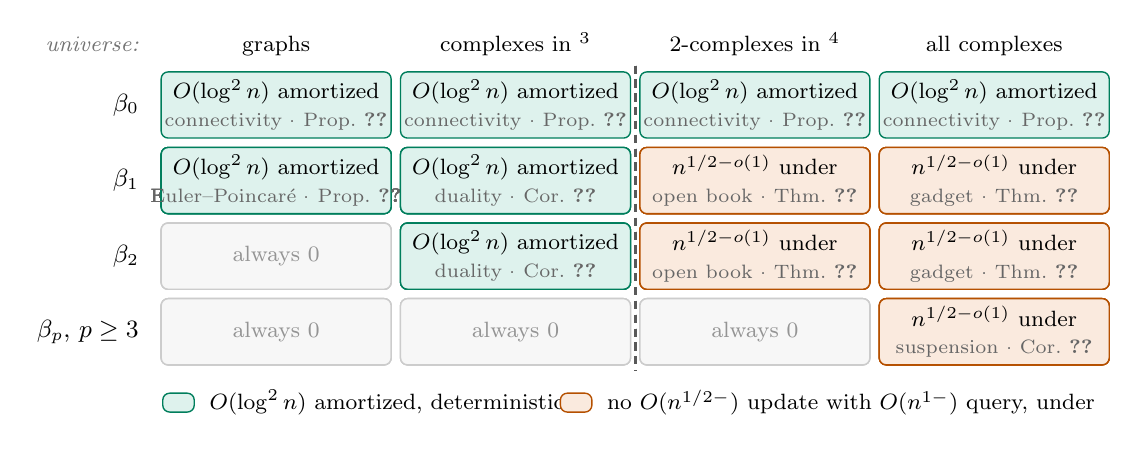
\begin{tikzpicture}[x=1cm,y=1cm,font=\footnotesize,
  cellbox/.style={rounded corners=2.5pt,line width=0.5pt},
  easy/.style={cellbox,fill=lsEasy!13,draw=lsEasy!80!black},
  hard/.style={cellbox,fill=lsHard!13,draw=lsHard!85!black},
  zero/.style={cellbox,fill=black!3,draw=black!20},
  hdr/.style={align=center,inner sep=1pt}]
  \def\cw{3.04}\def\ch{0.96}\def\gp{0.06}\def\xo{1.3}
  % \lscell{column}{row}{style}{bound}{method}{reference}
  \def\lscell#1#2#3#4#5#6{%
    \path[#3] ({\xo+#1*\cw+\gp},{-#2*\ch-\gp}) rectangle ({\xo+(#1+1)*\cw-\gp},{-(#2+1)*\ch+\gp});
    \node[align=center,inner sep=0pt] at ({\xo+(#1+0.5)*\cw},{-(#2+0.5)*\ch})
      {#4\\[0.6pt]{\scriptsize\color{black!60}#5\ \textperiodcentered\ #6}};}
  \def\lszero#1#2{%
    \path[zero] ({\xo+#1*\cw+\gp},{-#2*\ch-\gp}) rectangle ({\xo+(#1+1)*\cw-\gp},{-(#2+1)*\ch+\gp});
    \node[text=black!42] at ({\xo+(#1+0.5)*\cw},{-(#2+0.5)*\ch}) {always $0$};}
  % column headers: the class of the universe
  \foreach \c/\t in {0/{graphs},1/{complexes in $\R^3$},2/{$2$-complexes in $\R^4$},3/{all complexes}}
    \node[hdr,anchor=base] at ({\xo+(\c+0.5)*\cw},0.2) {\t};
  \node[anchor=base east,text=black!55,font=\footnotesize\itshape] at ({\xo-0.1},0.2) {universe:};
  % row headers
  \foreach \r/\t in {0/{$\beta_0$},1/{$\beta_1$},2/{$\beta_2$},3/{$\beta_{p}$, $p\ge3$}}
    \node[anchor=east] at ({\xo-0.1},{-(\r+0.5)*\ch}) {\small\t};
  % beta_0: dynamic connectivity, in every universe
  \foreach \c in {0,1,2,3} \lscell{\c}{0}{easy}{$O(\log^2 n)$ amortized}{connectivity}{Prop.~\ref{prop:beta0}}
  % beta_1
  \lscell{0}{1}{easy}{$O(\log^2 n)$ amortized}{Euler--Poincar\'e}{Prop.~\ref{prop:beta0}}
  \lscell{1}{1}{easy}{$O(\log^2 n)$ amortized}{duality}{Cor.~\ref{cor:anyR3}}
  \lscell{2}{1}{hard}{$n^{1/2-o(1)}$ under \OMv}{open book}{Thm.~\ref{thm:r4}}
  \lscell{3}{1}{hard}{$n^{1/2-o(1)}$ under \OMv}{gadget}{Thm.~\ref{thm:omv}}
  % beta_2
  \lszero{0}{2}
  \lscell{1}{2}{easy}{$O(\log^2 n)$ amortized}{duality}{Cor.~\ref{cor:anyR3}}
  \lscell{2}{2}{hard}{$n^{1/2-o(1)}$ under \OMv}{open book}{Thm.~\ref{thm:r4}}
  \lscell{3}{2}{hard}{$n^{1/2-o(1)}$ under \OMv}{gadget}{Thm.~\ref{thm:omv}}
  % beta_p, p >= 3
  \lszero{0}{3}
  \lszero{1}{3}
  \lszero{2}{3}
  \lscell{3}{3}{hard}{$n^{1/2-o(1)}$ under \OMv}{suspension}{Cor.~\ref{cor:allp}}
  % the dimension dichotomy between R^3 and R^4
  \draw[line width=1pt,black!65,dash pattern=on 3pt off 2pt] ({\xo+2*\cw},0.02) -- ({\xo+2*\cw},{-4*\ch-0.02});
  % legend, centred under the grid
  \begin{scope}[shift={({\xo+2*\cw},{-4*\ch-0.42})}]
    \path[easy] (-6.0,-0.12) rectangle (-5.6,0.12);
    \node[anchor=west] at (-5.53,0) {$O(\log^2 n)$ amortized, deterministic};
    \path[hard] (-0.95,-0.12) rectangle (-0.55,0.12);
    \node[anchor=west] at (-0.48,0) {no $O(n^{1/2-\eps})$ update with $O(n^{1-\eps})$ query, under \OMv};
  \end{scope}
\end{tikzpicture}
\caption{Maintaining one Betti number of a subcomplex~$K$ of a fixed universe with $n$ simplices under single-simplex insertions and deletions; the columns give the class of the universe.
Green: deterministic data structures with $O(\log^2 n)$ amortized update time and constant query time, after polynomial preprocessing.
Orange: assuming the \OMv\ conjecture, for every $\eps>0$ and over every field, no data structure with polynomial preprocessing time has amortized update time $O(n^{1/2-\eps})$ and query time $O(n^{1-\eps})$; over~$\Ftwo$, each of these problems is equivalent, up to constant factors, to dynamic matrix rank (Corollary~\ref{cor:equiv}, and Corollary~\ref{cor:r4-equiv} for~$\R^4$), and over every field the problems in the last column are equivalent to dynamic rank of $\{0,\pm1\}$-matrices.
The second line of a cell names the method: the \emph{gadget} of Section~\ref{sec:equiv}; the \emph{open book}, an explicit linear form of the embedding of Edelsbrunner and Parsa~\cite{EP14} applied to the gadget (Section~\ref{sec:lower-r4}); \emph{suspension}, which shifts Betti numbers up by one dimension (Lemma~\ref{lem:suspension}); and Alexander \emph{duality} (Section~\ref{sec:easy-s3}).
The dashed line marks the dichotomy between three and four dimensions; Table~\ref{tab:landscape} gives the precise bounds and further settings.}
\label{fig:landscape}
\end{figure}


\begin{table}[tb]
\caption{The bounds of Figure~\ref{fig:landscape} in detail, together with further settings. Updates are single-simplex insertions and deletions unless a row says otherwise. ``Amortized'' and ``worst-case'' refer to update time; the algorithms have query time $O(1)$ and polynomial preprocessing time, and the last two count field operations. Each lower bound holds for every $\eps>0$, over every field unless stated otherwise, and for every data structure with polynomial preprocessing time and query time $O(n^{1-\eps})$; the zigzag row instead bounds the total time of an online algorithm. Each lower bound assumes the \OMv\ conjecture, except the one marked~${}^{\dagger}$ in the last row, which assumes the \uMv-hinted \uMv\ conjecture of van den Brand, Nanongkai, and Saranurak~\cite{vdBNS19} and bounds the maximum of the update and query times; here $\alpha/2\ge5/8$, and $\alpha/2\approx0.703$ for the current bounds on rectangular matrix multiplication.}
\label{tab:landscape}
\small
\begin{tabular}{@{}>{\raggedright\arraybackslash}p{0.5\linewidth}ll@{}}
\toprule
\multicolumn{3}{@{}l}{\emph{Algorithms}}\\
\midrule
$\beta_0$, any universe & $O(\log^2 n)$ amortized & Prop.~\ref{prop:beta0} \\
All $\beta_p$, any fixed complex in $\R^3$ (polynomial preprocessing) & $O(\log^2 n)$ amortized & Cor.~\ref{cor:anyR3} \\
$\beta_p$ for fixed $p$, given a tree decomposition of the Hasse diagram of width $t$ & $O((t{+}1)^3\log n\log(t{+}2))$ worst-case & Cor.~\ref{cor:tw-betti} \\
All $\beta_p$, any universe (randomized) & $O(n^{1.407})$ worst-case & Cor.~\ref{cor:upper} \\
\midrule
\multicolumn{3}{@{}l}{\emph{Conditional lower bounds}}\\
\midrule
$\beta_p$ for any $p\ge1$ & $n^{1/2-o(1)}$ amortized & Cor.~\ref{cor:allp} \\
\quad\ldots\ on universes of bounded degree & $n^{1/2-o(1)}$ amortized & Sec.~\ref{sec:lower-bdeg} \\
\quad\ldots\ for $p\le2$, on universes linearly embedded in $\R^4$ & $n^{1/2-o(1)}$ amortized & Thm.~\ref{thm:r4} \\
\quad\ldots\ insertions only, or deletions only & $n^{1/2-o(1)}$ worst-case & Thm.~\ref{thm:partial} \\
Deciding $H_1(K)=0$, for connected $K$ with $\beta_1=\beta_2\le1$ & $n^{1/2-o(1)}$ amortized & Thm.~\ref{thm:acyclic} \\
Persistent Betti numbers under function-value updates & $n^{1/2-o(1)}$ amortized & Cor.~\ref{cor:persistence} \\
$\beta_p$ of clique and Vietoris--Rips complexes (metric spaces, points in $\R^{O(\log n)}$) & $n^{1/2-o(1)}$ amortized & Sec.~\ref{sec:flag} \\
Online zigzag persistence in degree one, length $L$ & $L^{3/2-o(1)}$ total & Cor.~\ref{cor:zigzag} \\
$\beta_p$ for any $p\ge1$ & $n^{\alpha/2-o(1)}$ worst-case${}^{\dagger}$ & Cor.~\ref{cor:hinted} \\
\bottomrule
\end{tabular}
\end{table}

\subsection{Technical overview}\label{sec:overview}


\paragraph{From homology to rank.}
For a complex $K$ and a field $\F$, the rank--nullity theorem gives
\[
  \beta_p(K)=n_p(K)-\rk\bd_p-\rk\bd_{p+1},
\]
where $n_p(K)$ is the number of $p$-simplices and $\bd_p$ is the $p$-th boundary matrix.
Inserting a $p$-simplex adds one column to~$\bd_p$; it does not change $\bd_{p+1}$, because no $(p+1)$-simplex containing it is present yet.
So a dynamic-rank structure for the boundary matrices of the universe, with absent simplices represented by zero columns, maintains every Betti number.

\paragraph{From rank to homology.}
Given a matrix $A\in\{0,1\}^{r\times k}$, we build a $2$-complex $\KA$ as follows (Figure~\ref{fig:gadget} and Definition~\ref{def:gadget}).
Row~$i$ becomes a \emph{row cycle}~$C_i$: three edges forming a hollow triangle.
Column~$j$ becomes a sphere with one hole per row, triangulated from constant-size pieces called \emph{sockets}.
The hole of row~$i$ is sealed by a single triangle if $A_{ij}=0$, and joined to $C_i$ by a tube of six triangles if $A_{ij}=1$.
The column therefore becomes a connected surface $\Sigma_j$ whose boundary consists of the row cycles $C_i$ with $A_{ij}=1$.
The key fact, Lemma~\ref{lem:crux}, is that a $2$-cycle has the same coefficient $x_j$ on every triangle of~$\Sigma_j$, because adjacent triangles must cancel along their common edge.
A $2$-chain with coefficient $x_j$ on every triangle of~$\Sigma_j$ has boundary $\sum_i\bigl(\sum_jA_{ij}x_j\bigr)C_i$, so it is a $2$-cycle exactly when $Ax=0$.
Hence the $2$-cycles correspond exactly to the vectors~$x$ with $Ax=0$, and $\beta_2(\KA)=k-\rk A$.
Flipping $A_{ij}$ exchanges the seal for the tube, which changes seven triangles.

\paragraph{Switches.}
Think of the columns of $A$ as unknowns and of the rows as equations.
A $2$-cycle puts a coefficient $x_j$ on~$\Sigma_j$, and for the boundary to cancel on $C_i$ these coefficients must satisfy the equation $\sum_jA_{ij}x_j=0$ of row~$i$.
If we insert the triangle that fills $C_i$, a $2$-cycle can cancel its boundary on $C_i$ with that triangle instead, and the equation of row~$i$ disappears: filling $C_i$ switches row~$i$ \emph{off}.
Columns work the other way around.
Each $\Sigma_j$ gets one more boundary component, a private hollow triangle $\Lambda_j$, the \emph{tether}, that no other surface touches.
While $\Lambda_j$ is hollow, nothing can cancel the boundary of $\Sigma_j$ there, so $x_j=0$ in every $2$-cycle; filling $\Lambda_j$ switches column~$j$ \emph{on}.
Each switch inserts or deletes a single triangle.
Now take $A=M\in\{0,1\}^{\ell\times\ell}$ and Boolean vectors $u,v\in\{0,1\}^{\ell}$ with supports $\supp u=\{i:u_i=1\}$ and $\supp v=\{j:v_j=1\}$.
If exactly the rows in $\supp u$ and the columns in $\supp v$ are on, then $\beta_2=\lvert\supp v\rvert-\rk M[\supp u,\supp v]$.
This is smaller than $\lvert\supp v\rvert$ exactly when $M[\supp u,\supp v]\ne0$, that is, exactly when the Boolean product $u^{\top}Mv=\bigvee_{i,j}u_iM_{ij}v_j$ equals~$1$; a $0/1$ matrix is nonzero over every field if it is nonzero at all, so this works over every field.
Answering $\ell$ such requests online is the \OuMv\ problem, which needs total time $\ell^{3-o(1)}$ under the \OMv\ conjecture, even after polynomial preprocessing of~$M$~\cite{HKNS15}.
Our universe has $n=\Theta(\ell^2)$ simplices, and moving from one request to the next takes $O(\ell)=O(\sqrt n)$ switches and one query.
A data structure with update time $n^{1/2-\eps}$ and query time $n^{1-\eps}$ would thus answer all $\ell$ requests in time $\ell\cdot(\ell\cdot\ell^{1-2\eps}+\ell^{2-2\eps})=O(\ell^{3-2\eps})$, contradicting the conjecture; this is where the exponents $1/2$ and $1$ in Theorem~\ref{thm:intro-omv} come from.

\paragraph{Almost no homology.}
The complexes above contain the whole $1$-skeleton of the universe, so their first Betti number is typically of order~$n$, and one might hope for algorithms whose cost depends on the homology rather than on the size of the complex.
To rule this out (Theorem~\ref{thm:acyclic}), we cone off the support graph of the matrix, which kills its cycles without changing the rank information.
We then encode an \OuMv\ request in a bordered matrix whose rank deficiency is a single bit, so that $\beta_1=\beta_2\in\{0,1\}$, and a standard random isolation step turns this bit into the Boolean answer.

\paragraph{Easy cases.}
For a proper subcomplex $K\subsetneq T$ of a triangulated $3$-sphere $T$, Alexander duality gives $\beta_2(K)=c-1$, where $c$ is the number of connected components of the complement of~$K$ in the sphere.
These components correspond to the components of a dual graph whose nodes are the tetrahedra of $T$ not in~$K$ and whose edges are the triangles of $T$ not in~$K$.
A simplex update changes this graph by $O(1)$ nodes or edges.
So $\beta_0$ and $\beta_2$ both reduce to dynamic connectivity, and the Euler--Poincar\'e formula gives~$\beta_1$.

\subsection{Organization}
% Figure: roadmap of the reductions and results.
% Requires tikz with the arrows.meta library. Okabe--Ito tints: core blue, hard orange, easy green.
\begin{figure}[t]
\centering
\providecommand{\uMv}{\textsf{uMv}}%
\providecommand\Description[2][]{}%
\Description{A flow diagram. On the left, three gray source boxes: the OMv conjecture, the uMv-hinted conjecture, and dynamic-rank algorithms. In the middle, two blue core boxes, dynamic rank and dynamic beta one, joined by arrows in both directions. On the right, a bracketed stack of nine orange boxes listing hard variants. Below a dashed line, three green boxes list the easy cases.}
\definecolor{rmCore}{HTML}{0072B2}%
\definecolor{rmHard}{HTML}{D55E00}%
\definecolor{rmEasy}{HTML}{009E73}%
\begin{tikzpicture}[x=1cm,y=1cm,font=\footnotesize,
  box/.style={rounded corners=2.5pt,line width=0.5pt,align=center,inner sep=2.5pt,minimum height=0.62cm},
  src/.style={box,fill=black!4,draw=black!45,text width=2.1cm,font=\small},
  core/.style={box,fill=rmCore!11,draw=rmCore!85!black,text width=2.45cm,minimum height=1.05cm,font=\small},
  hard/.style={rounded corners=2pt,line width=0.5pt,fill=rmHard!11,draw=rmHard!85!black},
  easy/.style={box,fill=rmEasy!11,draw=rmEasy!85!black},
  ref/.style={text=black!60,font=\scriptsize},
  arr/.style={-{Stealth[length=2.1mm,width=1.6mm]},line width=0.6pt,draw=black!70},
  lab/.style={font=\scriptsize,text=black!70,fill=white,inner sep=1pt}]
  % sources
  \node[src] (omv) at (1.1,1.05) {\OMv\\conjecture\\[-1pt]{\scriptsize\cite{HKNS15}}};
  \node[src] (hint) at (1.1,-0.65) {\uMv-hinted\\\uMv\\[-1pt]{\scriptsize\cite{vdBNS19}}};
  \node[src] (alg) at (1.1,-2.05) {dynamic-rank\\[-1pt]algorithms {\scriptsize\cite{San07,vdBNS19}}};
  % the core equivalence
  \node[core] (rank) at (4.45,0.05) {dynamic rank\\[-1pt]{\footnotesize flips + switches}};
  \node[core] (betti) at (7.65,0.05) {dynamic $\beta_1$\\[-1pt]{\footnotesize of $2$-complexes}};
  \draw[arr] (rank.20) -- node[lab,above=1.5pt] {gadget, Thm.~\ref{thm:equiv}} (betti.160);
  \draw[arr] (betti.200) -- node[lab,below=1.5pt] {Lem.~\ref{lem:betti-to-rank}} (rank.340);
  \draw[arr,rounded corners=3pt] (omv.east) -- node[lab,above=1pt,pos=0.5] {via \OuMv\ and switches, Thm.~\ref{thm:omv}} (7.15,1.05) -- (7.15,0.58);
  \draw[arr] (hint.east) -- (rank.195);
  % consequences (hard)
  \foreach \y/\t/\r in {
      2.0/{$\beta_p$ for every $p\ge1$}/{Cor.~\ref{cor:allp}},
      1.5/{bounded vertex degree}/{Thm.~\ref{thm:bdeg}},
      1.0/{$2$-complexes in $\R^4$}/{Thm.~\ref{thm:r4}},
      0.5/{partially dynamic}/{Thm.~\ref{thm:partial}},
      0.0/{deciding whether $H_1=0$}/{Thm.~\ref{thm:acyclic}},
      -0.5/{persistent Betti numbers}/{Cor.~\ref{cor:persistence}},
      -1.0/{Vietoris--Rips complexes}/{Thm.~\ref{thm:flag}},
      -1.5/{online zigzag persistence}/{Cor.~\ref{cor:zigzag}},
      -2.0/{worst case, every field}/{Cor.~\ref{cor:hinted}}} {
    \path[hard] (9.38,\y-0.21) rectangle (13.68,\y+0.21);
    \node[anchor=west,inner sep=0pt] at (9.47,\y) {\t};
    \node[anchor=east,inner sep=0pt,ref] at (13.61,\y) {\r};
  }
  \draw[line width=0.6pt,black!55] (9.3,2.21) -- (9.22,2.21) -- (9.22,-2.21) -- (9.3,-2.21);
  \draw[arr] (betti.east) -- (9.22,0.05);
  % algorithms transfer back
  \node[box,fill=rmCore!5,draw=rmCore!60,text width=2.75cm] (up) at (4.45,-2.05) {every $\beta_p$ in $O(n^{1.407})$\\[-1pt]{\scriptsize\color{black!60}worst case, Cor.~\ref{cor:upper}}};
  \draw[arr,dashed] (alg.east) -- (up.west);
  \draw[arr,dashed] (rank.south) -- node[lab,right=1pt] {Lem.~\ref{lem:betti-to-rank}} (up.north);
  % easy side
  \draw[black!25,line width=0.5pt,dash pattern=on 2pt off 2pt] (-0.05,-2.85) -- (13.65,-2.85);
  \node[font=\scriptsize\itshape,text=black!55,anchor=north west] at (-0.05,-2.9) {where maintenance is easy};
  \node[easy,text width=3.95cm] (b0) at (2.08,-3.65) {$\beta_0$; $\beta_1$ of graphs: $O(\log^2 n)$\\[-1pt]{\scriptsize\color{black!60}amortized; connectivity, Prop.~\ref{prop:beta0}}};
  \node[easy,text width=4.25cm] (r3) at (6.78,-3.65) {all $\beta_p$ in $\R^3$: $O(\log^2 n)$\\[-1pt]{\scriptsize\color{black!60}amortized; duality, Thm.~\ref{thm:s3}, Cor.~\ref{cor:anyR3}}};
  \node[easy,text width=4.25cm] (bw) at (11.48,-3.65) {$\beta_p$, constant treewidth: $O(\log n)$\\[-1pt]{\scriptsize\color{black!60}worst case; Cors.~\ref{cor:tw-betti} and~\ref{cor:bandwidth}}};
\end{tikzpicture}
\caption{Roadmap of the results. Solid arrows point in the direction in which hardness propagates; the two arrows between the core problems are the two halves of the equivalence (Theorem~\ref{thm:equiv}), and the \OMv\ lower bound is proved directly for Betti numbers, using the switches of the gadget. Dashed arrows transfer algorithms from dynamic rank to dynamic Betti numbers.
The orange boxes are the variants of the lower bound in Section~\ref{sec:lower}, listed in the order of Table~\ref{tab:landscape}; the pale box ``every $\beta_p$ in $O(n^{1.407})$'' is the general algorithm obtained from dynamic rank (Corollary~\ref{cor:upper}); the green boxes are the algorithms of Section~\ref{sec:easy}, where the treewidth is that of the Hasse diagram and the bandwidth bound is Corollary~\ref{cor:bandwidth}. The arrow from the hinted conjecture yields worst-case bounds only.}
\label{fig:roadmap}
\end{figure}

Figure~\ref{fig:roadmap} shows how the results depend on each other.
Section~\ref{sec:related} discusses related work.
Section~\ref{sec:prelim} fixes notation and defines the dynamic problems and the reductions we use.
Section~\ref{sec:equiv} presents the gadget and proves the equivalence.
Section~\ref{sec:lower} derives the conditional lower bounds and their variants, including the embedding of the hard universes in~$\R^4$.
Section~\ref{sec:easy} gives the algorithms for $\beta_0$, for subcomplexes of the $3$-sphere and of any fixed geometric complex in~$\R^3$, and for universes of small width or bounded treewidth.
Section~\ref{sec:conclusion} lists open problems.
